% Options for packages loaded elsewhere
\PassOptionsToPackage{unicode}{hyperref}
\PassOptionsToPackage{hyphens}{url}
\PassOptionsToPackage{dvipsnames,svgnames,x11names}{xcolor}
%
\documentclass[
  letterpaper,
  DIV=11,
  numbers=noendperiod]{scrartcl}

\usepackage{amsmath,amssymb}
\usepackage{iftex}
\ifPDFTeX
  \usepackage[T1]{fontenc}
  \usepackage[utf8]{inputenc}
  \usepackage{textcomp} % provide euro and other symbols
\else % if luatex or xetex
  \usepackage{unicode-math}
  \defaultfontfeatures{Scale=MatchLowercase}
  \defaultfontfeatures[\rmfamily]{Ligatures=TeX,Scale=1}
\fi
\usepackage{lmodern}
\ifPDFTeX\else  
    % xetex/luatex font selection
\fi
% Use upquote if available, for straight quotes in verbatim environments
\IfFileExists{upquote.sty}{\usepackage{upquote}}{}
\IfFileExists{microtype.sty}{% use microtype if available
  \usepackage[]{microtype}
  \UseMicrotypeSet[protrusion]{basicmath} % disable protrusion for tt fonts
}{}
\makeatletter
\@ifundefined{KOMAClassName}{% if non-KOMA class
  \IfFileExists{parskip.sty}{%
    \usepackage{parskip}
  }{% else
    \setlength{\parindent}{0pt}
    \setlength{\parskip}{6pt plus 2pt minus 1pt}}
}{% if KOMA class
  \KOMAoptions{parskip=half}}
\makeatother
\usepackage{xcolor}
\setlength{\emergencystretch}{3em} % prevent overfull lines
\setcounter{secnumdepth}{5}
% Make \paragraph and \subparagraph free-standing
\ifx\paragraph\undefined\else
  \let\oldparagraph\paragraph
  \renewcommand{\paragraph}[1]{\oldparagraph{#1}\mbox{}}
\fi
\ifx\subparagraph\undefined\else
  \let\oldsubparagraph\subparagraph
  \renewcommand{\subparagraph}[1]{\oldsubparagraph{#1}\mbox{}}
\fi


\providecommand{\tightlist}{%
  \setlength{\itemsep}{0pt}\setlength{\parskip}{0pt}}\usepackage{longtable,booktabs,array}
\usepackage{calc} % for calculating minipage widths
% Correct order of tables after \paragraph or \subparagraph
\usepackage{etoolbox}
\makeatletter
\patchcmd\longtable{\par}{\if@noskipsec\mbox{}\fi\par}{}{}
\makeatother
% Allow footnotes in longtable head/foot
\IfFileExists{footnotehyper.sty}{\usepackage{footnotehyper}}{\usepackage{footnote}}
\makesavenoteenv{longtable}
\usepackage{graphicx}
\makeatletter
\def\maxwidth{\ifdim\Gin@nat@width>\linewidth\linewidth\else\Gin@nat@width\fi}
\def\maxheight{\ifdim\Gin@nat@height>\textheight\textheight\else\Gin@nat@height\fi}
\makeatother
% Scale images if necessary, so that they will not overflow the page
% margins by default, and it is still possible to overwrite the defaults
% using explicit options in \includegraphics[width, height, ...]{}
\setkeys{Gin}{width=\maxwidth,height=\maxheight,keepaspectratio}
% Set default figure placement to htbp
\makeatletter
\def\fps@figure{htbp}
\makeatother

\KOMAoption{captions}{tableheading}
\makeatletter
\makeatother
\makeatletter
\makeatother
\makeatletter
\@ifpackageloaded{caption}{}{\usepackage{caption}}
\AtBeginDocument{%
\ifdefined\contentsname
  \renewcommand*\contentsname{Table of contents}
\else
  \newcommand\contentsname{Table of contents}
\fi
\ifdefined\listfigurename
  \renewcommand*\listfigurename{List of Figures}
\else
  \newcommand\listfigurename{List of Figures}
\fi
\ifdefined\listtablename
  \renewcommand*\listtablename{List of Tables}
\else
  \newcommand\listtablename{List of Tables}
\fi
\ifdefined\figurename
  \renewcommand*\figurename{Figure}
\else
  \newcommand\figurename{Figure}
\fi
\ifdefined\tablename
  \renewcommand*\tablename{Table}
\else
  \newcommand\tablename{Table}
\fi
}
\@ifpackageloaded{float}{}{\usepackage{float}}
\floatstyle{ruled}
\@ifundefined{c@chapter}{\newfloat{codelisting}{h}{lop}}{\newfloat{codelisting}{h}{lop}[chapter]}
\floatname{codelisting}{Listing}
\newcommand*\listoflistings{\listof{codelisting}{List of Listings}}
\makeatother
\makeatletter
\@ifpackageloaded{caption}{}{\usepackage{caption}}
\@ifpackageloaded{subcaption}{}{\usepackage{subcaption}}
\makeatother
\makeatletter
\@ifpackageloaded{tcolorbox}{}{\usepackage[skins,breakable]{tcolorbox}}
\makeatother
\makeatletter
\@ifundefined{shadecolor}{\definecolor{shadecolor}{rgb}{.97, .97, .97}}
\makeatother
\makeatletter
\makeatother
\makeatletter
\makeatother
\ifLuaTeX
  \usepackage{selnolig}  % disable illegal ligatures
\fi
\IfFileExists{bookmark.sty}{\usepackage{bookmark}}{\usepackage{hyperref}}
\IfFileExists{xurl.sty}{\usepackage{xurl}}{} % add URL line breaks if available
\urlstyle{same} % disable monospaced font for URLs
\hypersetup{
  pdftitle={FAQ},
  colorlinks=true,
  linkcolor={blue},
  filecolor={Maroon},
  citecolor={Blue},
  urlcolor={Blue},
  pdfcreator={LaTeX via pandoc}}

\title{FAQ}
\author{}
\date{}

\begin{document}
\maketitle
\ifdefined\Shaded\renewenvironment{Shaded}{\begin{tcolorbox}[sharp corners, interior hidden, boxrule=0pt, borderline west={3pt}{0pt}{shadecolor}, frame hidden, enhanced, breakable]}{\end{tcolorbox}}\fi

\renewcommand*\contentsname{Table of contents}
{
\hypersetup{linkcolor=}
\setcounter{tocdepth}{3}
\tableofcontents
}
\hypertarget{when-and-where-is-class}{%
\section{When and where is class?}\label{when-and-where-is-class}}

\subsection{Section 01 (Manbir Kaur)}

\begin{itemize}
\tightlist
\item
  When: Monday/Wednesday/Friday 9:25AM-10:40AM and Tuesday 1:20PM-4:00PM
\item
  Where: Sabin-Reed 308
\end{itemize}

\subsection{Section 02 (Casey Berger)}

\begin{itemize}
\tightlist
\item
  When: Monday 1:40PM-2:55PM, Wednesday/Friday 1:20PM-2:35PM, and
  Tuesday 1:20PM-4:00PM
\item
  Where: Sabin-Reed 305
\end{itemize}

\hypertarget{where-do-i-get-my-textbook}{%
\section{Where do I get my textbook?}\label{where-do-i-get-my-textbook}}

First: \textbf{do not buy a copy of the book} -- it's available to
borrow for the entire semester from Nielsen Library. Please ask for
``Physicists for Scientists and Engineers'' or just ``the textbook for
PHY 117'' at the front desk.

If you decide you love this textbook so much that you would like to buy
a copy for yourself to keep forever, of course feel free to do so. But
we strongly recommend that you not do that.

\hypertarget{officehours}{%
\section{When are your office hours?}\label{officehours}}

\subsection{Casey}

Office hours:

\begin{itemize}
\tightlist
\item
  in-person (McConnell 301A): TBD
\item
  \href{https://smith.zoom.us/j/98280229454}{zoom}: TBD
\item
  by appointment: see Moodle for a link to my calendly page and schedule
  an appointment
\end{itemize}

\subsection{Manbir}

\hypertarget{duedates}{%
\section{When is \_\_ due?}\label{duedates}}

You can find all due dates on the
\href{https://docs.google.com/spreadsheets/d/1NN6zv30J_MdUYzjDmjOMn1q-IKhxN0H8w9O3rMQsQ1A/edit?usp=sharing}{course
schedule}. Dates are subject to change, but will always be kept up to
date on the schedule so check back if you're not sure.

\hypertarget{extensionpolicy}{%
\section{Can I have an extension?}\label{extensionpolicy}}

In general, we are happy to work with you on deadlines, but it's
important for you to communicate with us. You can request extensions
using \href{https://forms.gle/qTLy66bkUNZ5ibTj7}{this form}. Please note
that the 48 hour extension is automatically granted, while anything
longer than that requires that we have a conversation. That conversation
starts by you proposing a new deadline in the form, and then your
instructor can talk to you about what's possible or reasonable given the
course schedule, your circumstances, and other factors that may vary as
the semester progresses.

For more on our deadlines and extension policy, see the
\href{syllabus.qmd\#deadlines}{syllabus}.

\hypertarget{revisionpolicy}{%
\section{Can I revise and resubmit something I did poorly
on?}\label{revisionpolicy}}

For most assignments, yes. Some assignments cannot be revised or retaken
because of the nature of the assignment or when it is due. More
information for each assignment can be found on this
\href{https://docs.google.com/spreadsheets/d/1o43gE7XIsHia5bAcqoeek3scpJ-EyI1tOqB7SRFVZX0/edit?usp=sharing}{template
grade sheet}.

\hypertarget{emails}{%
\section{When will you reply to my email?}\label{emails}}

Timely communication is really important, but in order to be effective
instructors, we also need to be able to take breaks from email. Here are
the expectations you can have of us with respect to email response time:

\subsection{Casey}

If you email me on a weekday, you can expect a response from me within
24 hours. If you email me on a weekend, you can expect a response from
me by class time on Monday (or the first day back if it's a long weekend
or holiday).

\subsection{Manbir}

\hypertarget{gradingcurve}{%
\section{Do you grade on a curve?}\label{gradingcurve}}

Grades are not curved; your grade depends only on your own performance,
supporting your fellow students will help every one of you.

Your grades can be calculated using our
\href{https://docs.google.com/spreadsheets/d/1o43gE7XIsHia5bAcqoeek3scpJ-EyI1tOqB7SRFVZX0/edit?usp=sharing}{template
grading sheet}, and letter grades are determined from percentages using
\href{syllabus.qmd\#lettergrades}{this chart}

\hypertarget{cornellnotes}{%
\section{What the heck are Cornell Notes??}\label{cornellnotes}}

Cornell Notes are a method of structuring your note-taking to improve
comprehension and retention.

The goal of Cornell Notes is not just good in-class note-taking, but
developing a short but effective regular review process. To do this, you
divide your page into four blocks, as shown below.

\begin{figure}

{\centering 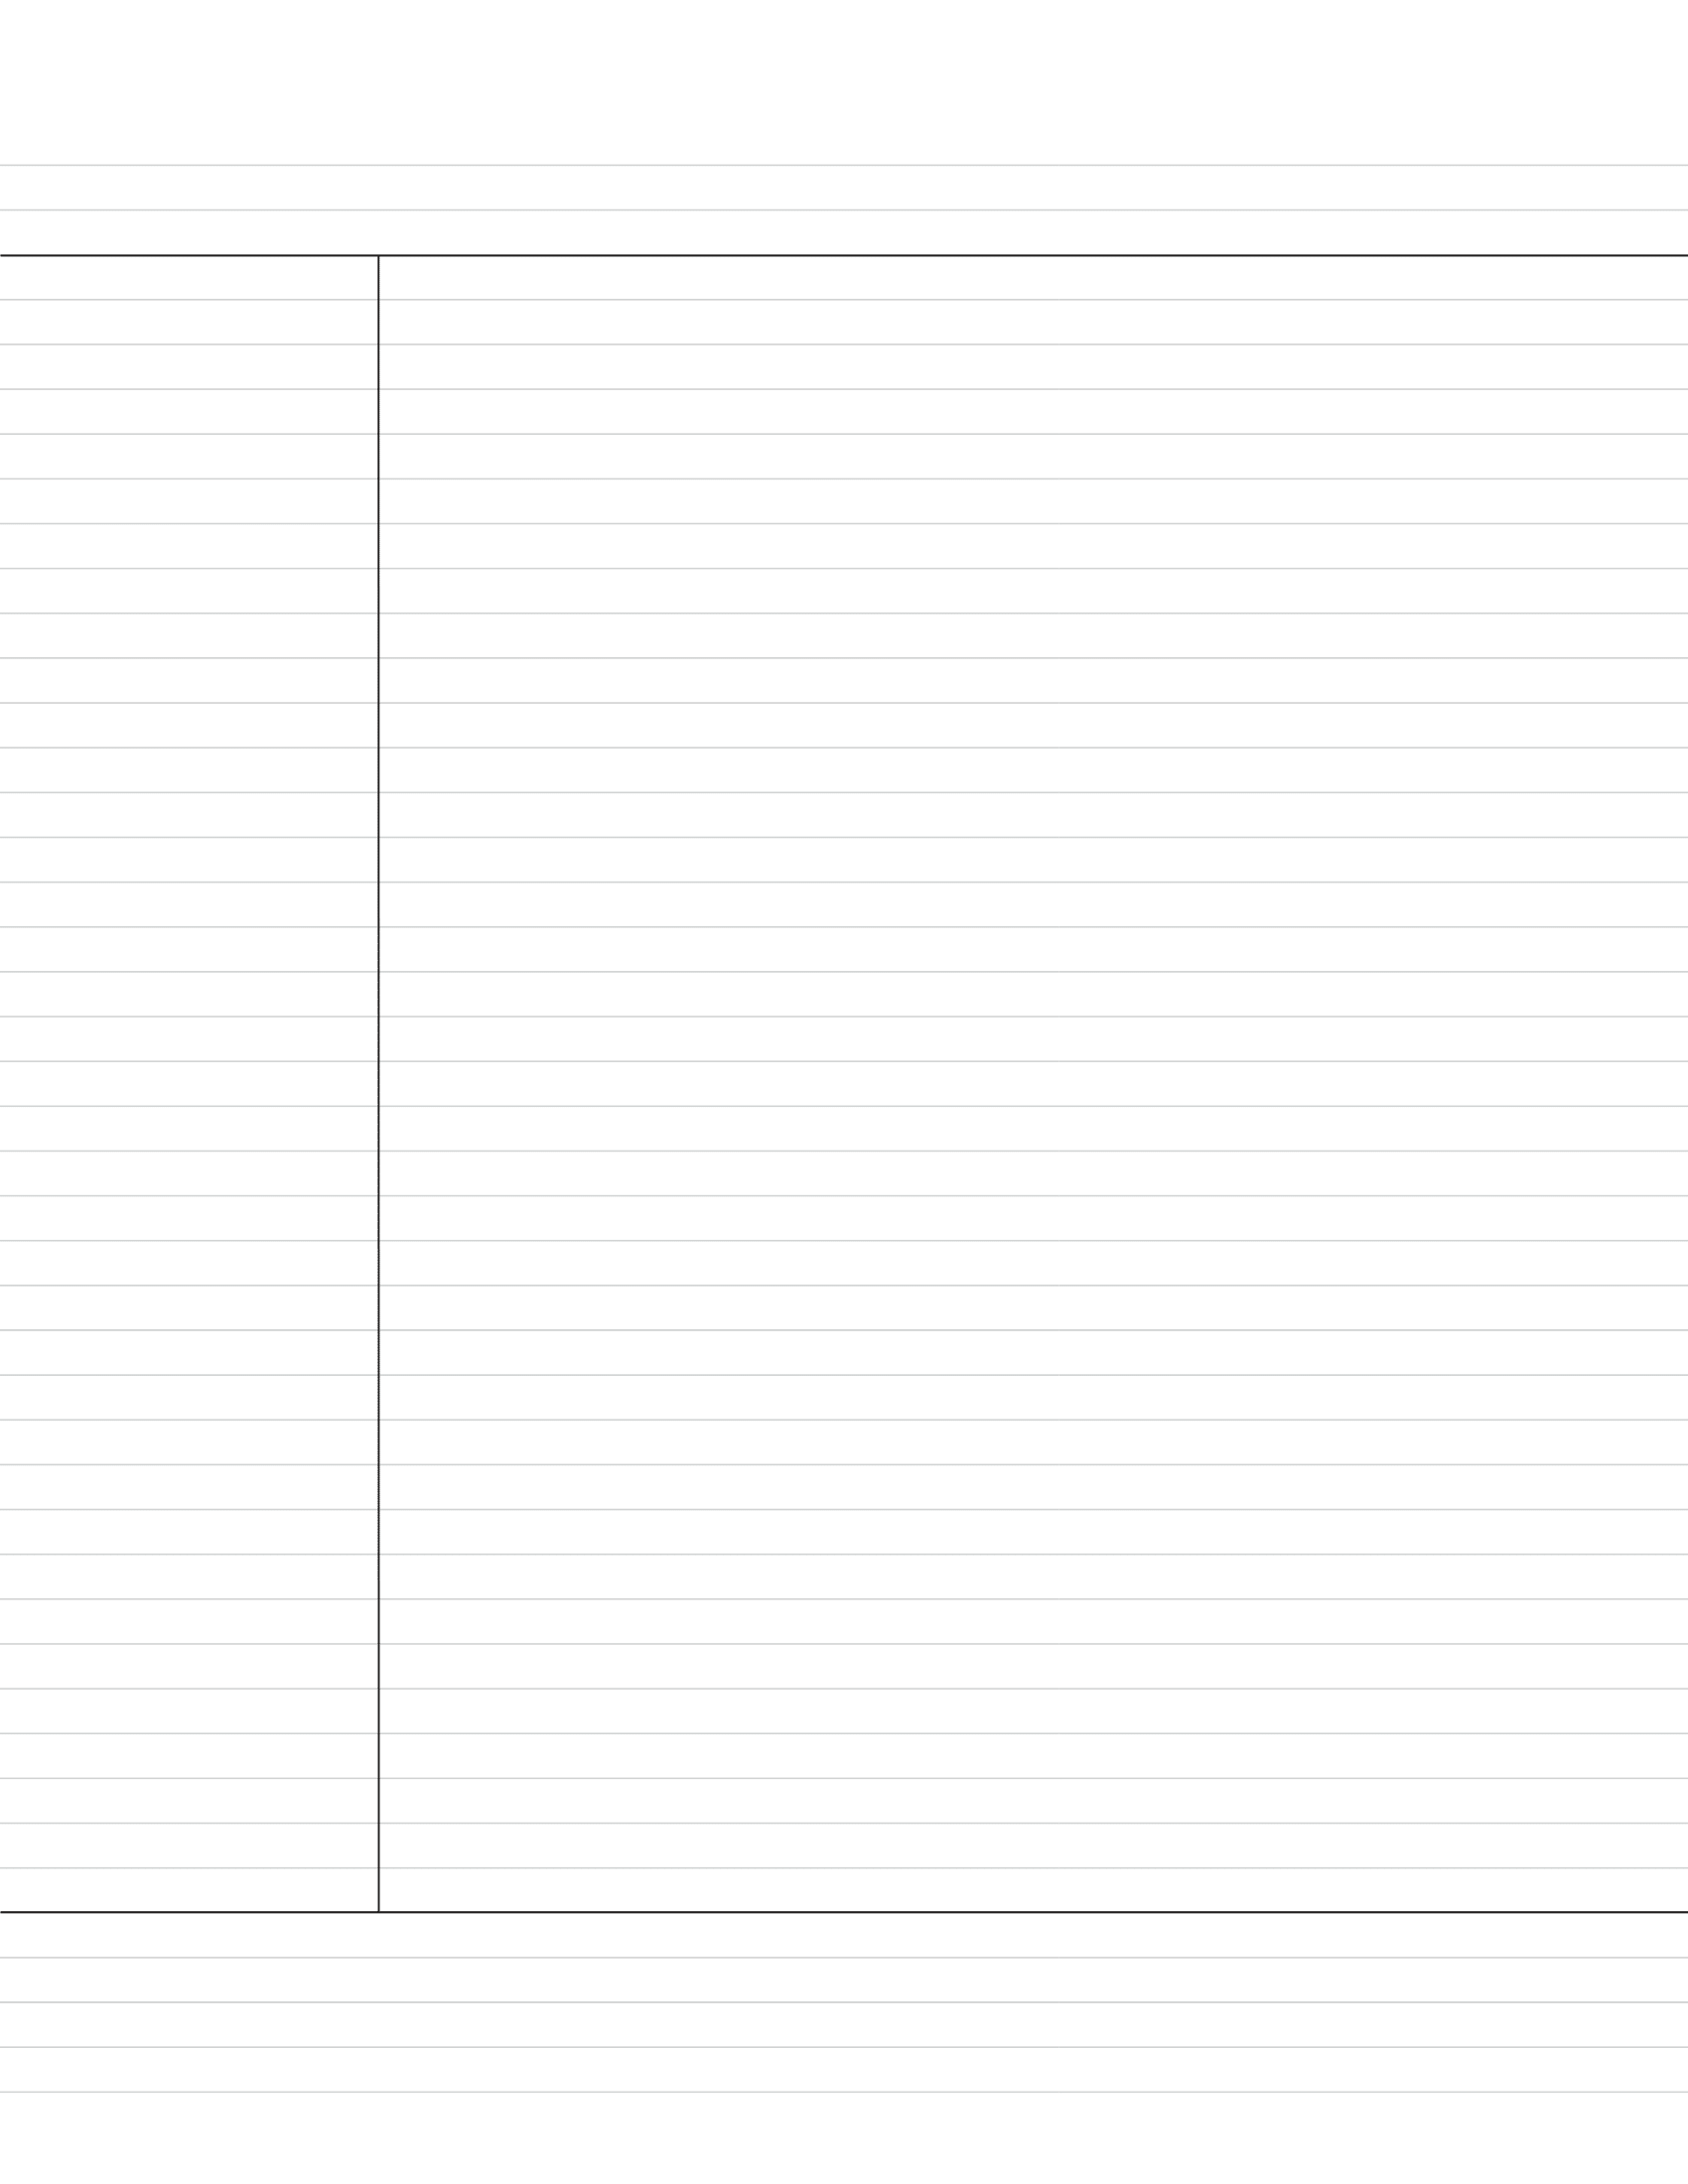
\includegraphics{graphics/CornellNotes0.pdf}

}

\caption{Cornell notes initial setup}

\end{figure}

Each of these four spaces has a purpose:

\begin{itemize}
\tightlist
\item
  The header is where you write the topic: in just a few words, what is
  this lesson about?
\item
  The largest section is for taking notes during class, just as you'd
  always take notes
\item
  The sidebar on the left is where you write cues or questions about the
  content
\item
  The footer is where you write a brief (one-sentence) summary of the
  page's content
\end{itemize}

The process for doing this can be divided into three steps:

\subsection{During class}

During class, you fill out the topic and take notes in the largest
space, as shown here 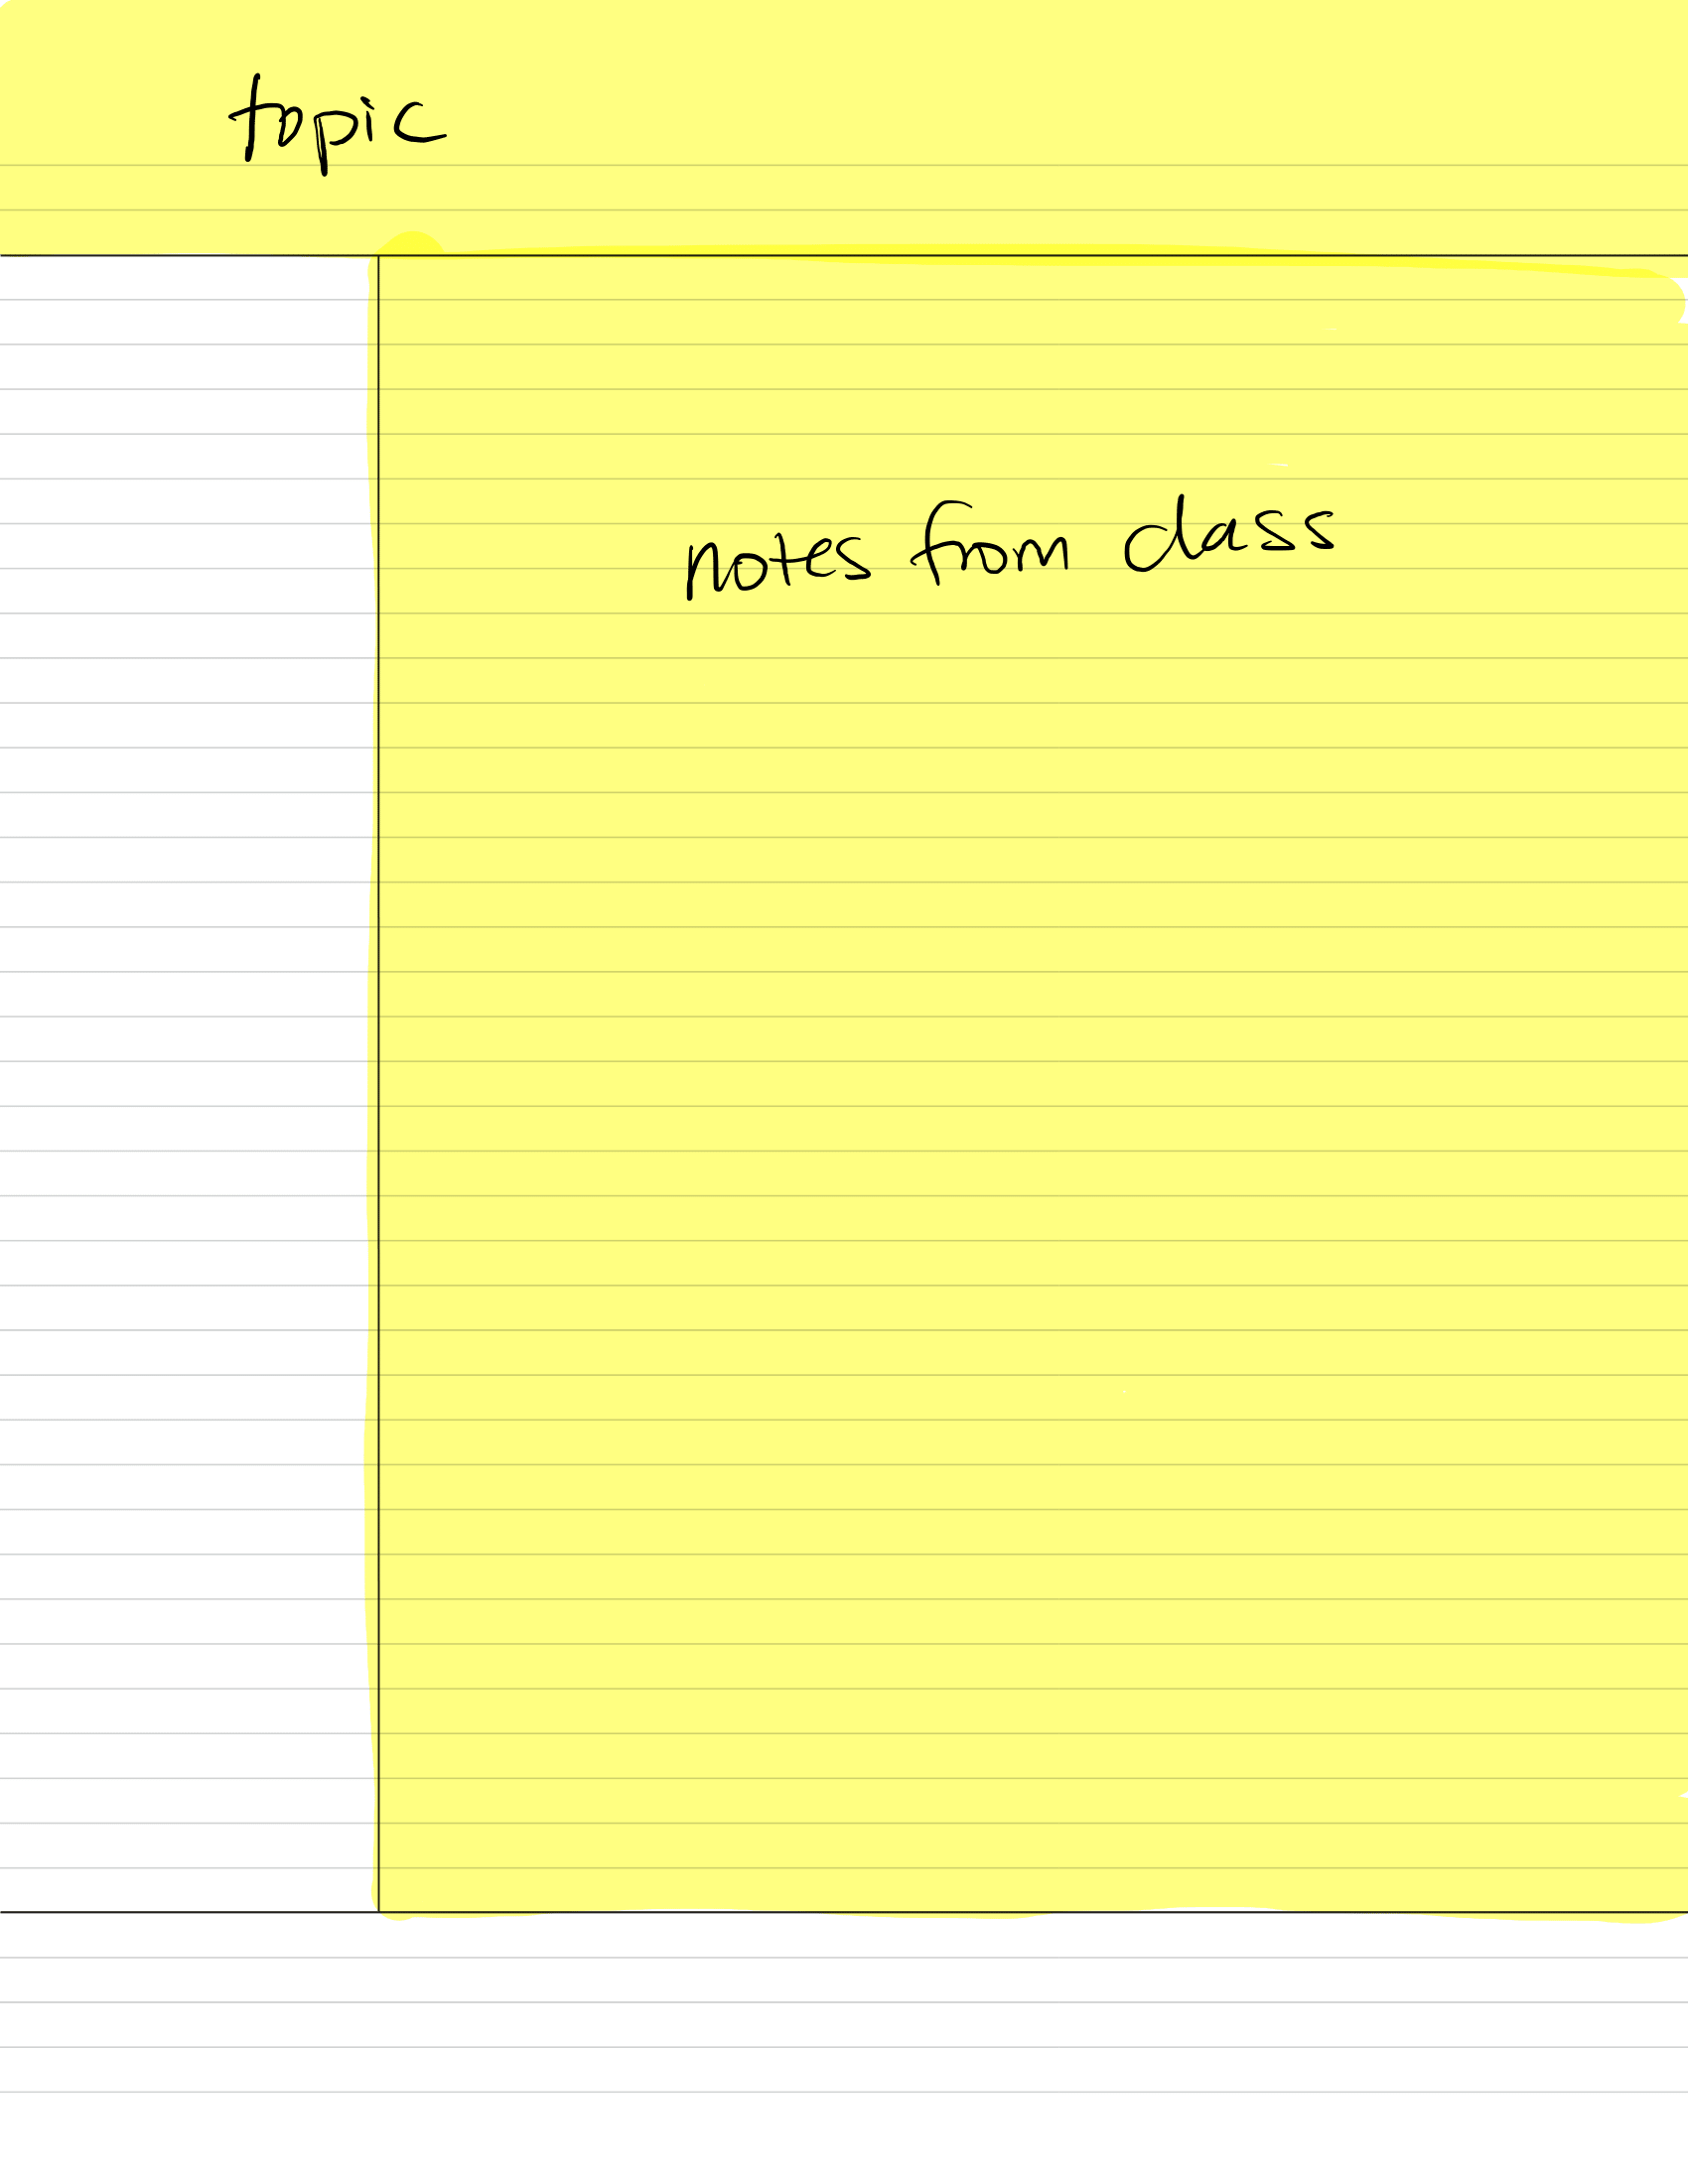
\includegraphics{graphics/CornellNotes1.pdf} \#\#\#
Later that day

\subsection{Later that week}

\hypertarget{ChatGPT}{%
\section{Can I use ChatGPT in this class?}\label{ChatGPT}}

\hypertarget{catchingup}{%
\section{What should I do if I get behind on my
work?}\label{catchingup}}

First, reach out to your instructor. It helps us to know that you are
working on catching up. We are also happy to meet and help you set
adjusted deadlines to get back on track.

Second, if you are feeling really overwhelmed, consider scheduling an
appointment with
\href{https://go.oncehub.com/LearningSpecialistDuncanGriffin}{Duncan
Griffin} at the Jacobson Center. His role is to support students seeking
help with time management, organization, reading, test-taking,
note-taking, and other academic skills. He can help you talk through
what strategies work for you, what strategies don't, and how to manage
your time and energy in a more sustainable way.

\hypertarget{ODS}{%
\section{I have accommodations from ODS. What should I do?}\label{ODS}}

We have tried to bring the concept of
\href{https://www.washington.edu/doit/what-universal-design-0}{universal
design} into how we have planned and structured this course, so we hope
that any accommodations you have from ODS are already built into this
course. However, we don't expect to have done this perfectly (as there
is no such thing), so if you have need of certain accommodations that
are not already provided by this class, please let us know and we will
do our best to meet those needs.



\end{document}
